%%%%%%%%%%%%%%%%%%%%%%%%%%%%%%%%%%%%%%%%%%%%%%%%%%%%%%%%%%%%%%%%%%%%%
% PREAMBLE
%%%%%%%%%%%%%%%%%%%%%%%%%%%%%%%%%%%%%%%%%%%%%%%%%%%%%%%%%%%%%%%%%%%%%

%% Start with one of the following:
% DOUBLE-SPACED VERSION FOR SUBMISSION TO THE AMS
\documentclass{ametsoc}

% TWO-COLUMN JOURNAL PAGE LAYOUT---FOR AUTHOR USE ONLY
% \documentclass[twocol]{ametsoc}

%%%%%%%%%%%%%%%%%%%%%%%%%%%%%%%%
%%% To be entered only if twocol option is used

\journal{jpo}

%  Please choose a journal abbreviation to use above from the following list:
% 
%   jamc     (Journal of Applied Meteorology and Climatology)
%   jtech     (Journal of Atmospheric and Oceanic Technology)
%   jhm      (Journal of Hydrometeorology)
%   jpo     (Journal of Physical Oceanography)
%   jas      (Journal of Atmospheric Sciences)	
%   jcli      (Journal of Climate)
%   mwr      (Monthly Weather Review)
%   wcas      (Weather, Climate, and Society)
%   waf       (Weather and Forecasting)
%   bams (Bulletin of the American Meteorological Society)
%   ei    (Earth Interactions)

%%%%%%%%%%%%%%%%%%%%%%%%%%%%%%%%
%Citations should be of the form ``author year''  not ``author, year''
\bibpunct{(}{)}{;}{a}{}{,}

%%%%%%%%%%%%%%%%%%%%%%%%%%%%%%%%

%%% To be entered by author:

%% May use \\ to break lines in title:

\title{Barotropic vorticity balance of the North Atlantic subpolar gyre in a strongly eddying model}

%%% Enter authors' names, as you see in this example:
%%% Use \correspondingauthor{} and \thanks{Current Affiliation:...}
%%% immediately following the appropriate author.
%%%
%%% Note that the \correspondingauthor{} command is NECESSARY.
%%% The \thanks{} commands are OPTIONAL.

    %\authors{Author One\correspondingauthor{Author One, 
    % American Meteorological Society, 
    % 45 Beacon St., Boston, MA 02108.}
% and Author Two\thanks{Current affiliation: American Meteorological Society, 
    % 45 Beacon St., Boston, MA 02108.}}

\authors{M. Lecorre\correspondingauthor{Laboratoire d’Oc\'eanographie Physique et Spatiale (LOPS), IUEM, Brest, France.}, J. Gula, and A.-M. Tr\'eguier}

%% Follow this form:
    % \affiliation{American Meteorological Society, 
    % Boston, Massachusetts.}

\affiliation{Univ. Brest, CNRS, IRD, Ifremer, Laboratoire d’Océanographie Physique et Spatiale (LOPS), IUEM, Brest, France}

%% Follow this form:
    %\email{latex@ametsoc.org}

\email{mathieu.lecorre@univ-brest.fr}

%% If appropriate, add additional authors, different affiliations:
    %\extraauthor{Extra Author}
    %\extraaffil{Affiliation, City, State/Province, Country}

  
%\extraauthor{}
%\extraaffil{}

%% May repeat for a additional authors/affiliations:

%\extraauthor{}
%\extraaffil{}

%%%%%%%%%%%%%%%%%%%%%%%%%%%%%%%%%%%%%%%%%%%%%%%%%%%%%%%%%%%%%%%%%%%%%
% ABSTRACT
%
% Enter your abstract here
% Abstracts should not exceed 250 words in length!
%
% For BAMS authors only: If your article requires a Capsule Summary, please place the capsule text at the end of your abstract
% and identify it as the capsule. Example: This is the end of the abstract. (Capsule Summary) This is the capsule summary. 

\abstract{hihi}

\begin{document}


\section{Barotropic vorticity balance}

\subsection{An overall view of the subpolar gyre balance}

To study the dynamic of the gyre we choose to compute the barotropic vorticity equation, this equation consist on integrating the momentum equations in the vertical and cross-differentiating them. The difference with looking at the barotropic potential vorticity equation, which can be find when averaging the vertical velocity, is that we have informations on how the barotropic vorticity is conserved while barotropic PV gives intel on what are the main contributor for making the flow leaves the $\frac{f}{h}$ lines.

The interaction of the flow with the sloping topography gives rise to the bottom pressure torque, which plays a key role in the barotropic vorticity equilibrium of the subpolar gyre (fig \ref{spatial_BV}). The full barotropic vorticity equation is given as follow \citep{gula2015}:

$$\underbrace{\frac{\partial \Omega}{\partial t}}_{rate} = -\underbrace{\nabla.(f\overline{u})}_{planet.vort.adv}+\underbrace{\frac{J(P_b,h)}{\rho _0}}_{bot.pres.torque} +\underbrace{k.\nabla \times \frac{\tau _{wind}}{\rho_{0}}}_{wind.curl} -\underbrace{k.\nabla \times \frac{\tau _{bot}}{\rho_{0}}}_{bot.drag.curl} +\underbrace{D_{\Sigma}}_{horiz.diffusion}-\underbrace{A_{\Sigma}}_{NL advection}$$

where the vorticity is the curl of the vertically integrated component of the velocity between the bottom and the surface. The non linear term can be written as:


$$A_{\Sigma}= \frac{\partial ^2 (\overline{vv}-\overline{uu})}{\partial x \partial y}+\frac{\partial ^2 \overline{uv}}{\partial x \partial x} -\frac{\partial ^2 \overline{uv}}{\partial y \partial y}$$

where (u,v) denote the horizontal components of the flow in (x,y) directions and the overbar defines a vertically integrated quantity:

$$\overline{u}=\int^{\eta}_{-h} u dz$$

with $\eta(x,y,t)$ the free surface height and $h(x,y)$ the topography. The bottom pressure torque J(P$_b$,h) is the Jacobian of the bottom pressure and the depth of the topography. In an idealized case of a geostrophic current flowing along a topography in free-slip condition the BPT can be written $\frac{J(P_b,h)}{\rho _0}=f u_b.\nabla h$. Given the kinematic condition at the bottom we have $-u_b . \nabla h =w_b$, the BPT can be then written $\frac{J(P_b,h)}{\rho _0}=-fw_b$ which means that when the flow tries to cross isobath by having a vertical velocity, the topography counterbalanced by generating a torque to return the flow along the isobath. In the same way it is possible to decompose $-\nabla.(f\overline{u})=-\beta \overline{V}-f \frac{\partial \eta}{\partial t}$. As we take the mean on a long time period $\frac{\partial \eta}{\partial t} \approx 0$ we write  $-\nabla.(f\overline{u})= - \beta \overline{V}$

The barotropic vorticity terms have been computed for the North Atlantic using different models (OGCM, POP) at different resolutions ($1^{\circ}$, $0.25^{\circ}$, $0.1^{\circ}$) in \citet{hughes2001} and \citet{yeager2015} . Their major result is that the barotropic vorticity balance in both gyres is mainly a balance between $\beta$V, $\nabla \times \frac{\tau _{wind}}{\rho_{0}}$ and $\frac{J(P_b,h)}{\rho _0}$. When the resolution of the model is increased from $1^{\circ}$ to $0.1^{\circ}$ in \citet{yeager2015}, there is no real impact for these three terms, but there is an increase of the amplitude of the non linear term, mostly in the Gulf Stream and NAC regions, and a decrease of the amplitude of the viscous torque in the boundary currents.

The major difference with the previous works is that some terms, such as the the BPT or the planetary vorticity, are at least one order of magnitude higher locally. This difference can go up to 3 orders of magnitude for the Non Linear Advection (NLA) term compared to the $0.1^{\circ}$ simulation of \citet{yeager2015}. The curl of the wind stress has the same pattern in each model. It is mostly positive with the strongest signal on the East of Greenland. The terms with the largest amplitudes are BPT and NL. Both exhibit small scale signals linked to the local variation of the topography, but compensate well with each other. Their sum $\frac{J(P_b,h)}{\rho _0}-A_{\Sigma}$ is of the same order of magnitude than the $\beta$V and Bottom Drag Curl (BDC). In our simulation, the amplitude of the $\beta$V term is also stronger than simulations at lower resolution. In the simulations of  \citet{hughes2001} and \citet{yeager2015}, the patterns of the $\beta$V term showed that the currents were much wider, reaching the interior of the gyre. Here, the patterns shows the presence of thinner and more intense currents, closely following the continental slopes.


In our simulations, the amplitude of the diffusion term due to vicosity effect ($D_{\Sigma}$) is small while the amplitude of the BDC is comparable to $\beta V$, the opposite happens in Yeager experiments. Surprisingly, his viscosity and our drag are quite similar both in pattern and in amplitude which would imply a change in the processes near the topography due to the choice of vertical coordinate. The z-levels coordinates have vertical walls between each level which increases the viscosity effect and explain the pattern in Yeager, while the $\sigma$-levels coordinates are close to inviscid boundary current with dissipation due to the stress at the bottom instead of having a viscous layer. We can note that the viscosity parametrisation  in z-levels coordinates is doing a good job in reproducing physical dissipation due to the bottom stress.


Spatial integrations are performed inside the gyre (fig \ref{intgyre_BV})to understand what are the main contributors of the circulation in the subpolar gyre. We can check that the term $\beta$V integrates to zero as we chose close contours.

Using oxygen isotope \citet{chapman1986,chapman1989} shown there is a connection from West Greenland toward the Mid-Atlantic Bight (North of Cap Hatteras) by a shelf current. This alongshelf flow is independant of the mean wind and is buoyancy driven \citep{csanady1978}. The subpolar gyre seems to act as a boundary that isolated the shelf and making it independant from its circulation. 

We perform integration of the barotropic vorticity equation in the subpolar gyre for the 0 Sv and the -3 Sv contours (fig \ref{intgyre_BV}). The 0 Sv contour tends to overlap the upper slope and the shelf (especially along West Greenland and East Canada) while the -3 Sv contour does not take into account the shelves. There is a change in the dynamic of the gyre depending of the contour we choose.

By taking the integration over the -3 Sv (which means excluding the shelf area), the main sources for the cyclonic circulation of the gyre are the wind and the BPT. They are balanced by the BDC. The signal of the wind does not contribute much locally, but becomes significant when spatially integrated over the gyre. The BPT is the major source of positive vorticity and helps the flow moves cyclonicaly around the gyre. The major sinks of vorticity are the NLA and the BDC. The BDC is very intense where the flow is close to a steep topography, as in the case of the Western Labrador Sea Current (WLSC) and the Western Greenland Current but also near the CGFZ. 

Like in the -3 Sv integration, the wind is a major contributor for the cyclonic circulation and the BDC represent the major sink of vorticity. In the 0 Sv the NL term substitutes the BPT for input of vorticity into the gyre. In this interpretation the wind forces the gyre cyclonicaly and the NL term helps to redistribute the vorticity inside it while the drag balance this input along steep topography. 

In the difference which cover the upper slope and the shelf the dynamic is different with a wind contribution being small and a balance between BPT, NLA and bottom drag. This balance is close to the one describe in \citet{csanady1978} and evokes a buoyancy driven flow in this area. 

This result seems to be coherent with previous work with a different dynamic in shallow water. Following the idea of Chapman 86-89 were the shelf does not interact with the subpolar gyre, it feels natural to exclude the upper slope and the shelf from our study. To do so in the following we will focus on the -3 Sv contour which is the biggest close domain excluding the boundary.
 
To better understand the pattern terms in the -3 Sv contour, we further divide the domain into an inner and boundary part as represented in fig. \ref{int_bound_inner_BV}. The two domains are defined using the -3 Sv line as previously, and the 3000 m isobath. What is between the -3 Sv line and the 3000m isobath is considered as the boundary zone and the rest is considered as the inner zone. The choice of the 3000 isobath is purely subjective but the results are consistent if we choose different contours inside the -3 Sv contour. 

In the boundary zone, the main source of cyclonic vorticity is the BPT. Secondary sources are the curl of the wind and the $\beta$V. The negative NL term sign indicates a vorticity advection outside of this domain which might either be the shelf or the inner gyre.

%In comparison, in the low resolution simulation (not shown) most of the vorticity dissipated locally by the BDC, while the high resolution vorticity is advected inside. 

In the inner zone, the NLA term represents the major contribution to the cyclonic circulation. It is balanced by the BDC, the BPT and the $\beta$V terms. Contributions from the BDC are of similar magnitude in the inner and boundary zones. The inner part of the gyre in not in Sverdrup balance at the first order, which would imply a dominant balance between a negative $\beta$V and a positive input from the curl of the wind stress. The wind input of vorticity is smaller than in the boundary zone, as the major wind source of vorticity is located along the Greenland area (fig \ref{spatial_BV}) and not uniformly distributed over the gyre.

The comparison between balances in the inner and boundary zones seems to indicate that the NLA term helps to redistribute vorticity from the boundary toward the interior of the gyre. The cyclonic vorticity is provided by the BPT at the boundaries of the gyre, and balanced by a sink of positive vorticity by the BDC all over the gyre.

\subsection{Characterisation of the Non Linear advective term}


The Non linear advective term is obtained by taking the curl of the vertically integrated momentum equation. The NL term is locally important and balance the bottom pressure torque around seamounts. When integrated over the gyre it seems to play a role in advecting the barotropic vorticity from the boundary toward the inside of the gyre. This component is quite difficult to interpret as many processes are hidden inside it. By decomposing the velocity in a barotropic and baroclinic part ($u = \overline{u} + u'$) the NL advection term can be written as follow:

$$A_{\Sigma}=\underbrace{A(\overline{u},\overline{v})}_{A^{bt}_{\Sigma}}+\underbrace{A(u',v')}_{A^{bc}_{\Sigma}}$$


where the barotropic part can be written as $A(\overline{u},\overline{v})= \overline{u}\Omega _x +\overline{v}\Omega _y$ which is the advection of the barotropic vorticity by the barotropic flow.  When integrated over the interior (Fig \ref)the contribution is evenly divided between barotropic and baroclinic contribution. It appears that the baroclinic contribution is mainly given by the NWC. Considering that the export of barotropic vorticity by baroclinic NL term along the topography is rather small, the remaining part might come from the South-Eastern boundary. In the boundary area the barotropic contribution is the dominant one. Considering the need from the inner part, the boundary value is too high meaning that a large quantity of the mean NL advection term only helps locally for the balance of the boundary current. The remaining part is used to export of barotropic vorticity inside the gyre. 

%where the barotropic part can be written as $A(\overline{u},\overline{v})= \overline{u}\Omega _x +\overline{v}\Omega _y$ which is the advection of the barotropic vorticity by the barotropic flow. When integrated (Fig \ref{int_NL}), the barotropic contribution count for almost all the export of barotropic vorticity. This is coherent with studies showing that most of the currents in our boundary area are mainly barotropic \citep{vanaken1995,daniault2011,lozier2017}. Surprisingly the inner part of the gyre is different with barotropic and baroclinic components being of similar amplitudes. After discrediting the inner part (not shown), we figured out that half of the baroclinic signal comes from the presence of the NAC in the South-western part of the domain.

It is also possible to decompose the NL term into a mean and eddy part by writing $u = \langle u \rangle + u^*$ where $\langle \bullet\rangle$ is the time average and the star denote the fluctuation part. By putting this in the non linear operator $A_{\Sigma}$ we have:

$$A_{\Sigma}(u,v)=\underbrace{A_{\Sigma}(\langle u \rangle, \langle v \rangle)}_{A_{\Sigma}^{mean}} + \underbrace{A_{\Sigma}(u^*,v^*)}_{A_{\Sigma}^{eddy}} +\underbrace{\langle  2\frac{\partial ^2 \overline{\langle v \rangle v^*} -\overline{\langle u \rangle u^*}}{\partial xy} +\frac{\partial ^2 \overline{\langle u \rangle v^*} + \overline{\langle v \rangle u^*}}{\partial xx} - \frac{\partial ^2 \overline{\langle u \rangle v^*} +\overline{ \langle v \rangle u^*}}{\partial yy}\rangle}_{\varepsilon}$$

Where the $\varepsilon$ part being the residue of the cross product and its value is negligible compared to both mean and eddy part. When integrated over the boundary area, the eddy component dominates over the mean one. In the inner part, the supply of barotropic vorticity is mainly linked to the eddy component but the mean component is also non negligible. More specifically most of mean signal is coming from the NWC, this being consistent with the result from \citet{wang2017}. Taking into account that the NWC covers most of the need for the for the mean signal, the signal generated inside the boundary might be used for the shelf dynamics among other things. Also, vorticity advection by eddies generated along the boundary area is too large compared to what is needed by the interior (when excluding the NWC), the leftover is advecting barotropic vorticity outside of the domains. 


We can identify several processes for providing barotropic vorticity to the subpolar gyre. The most important is the eddy contribution coming from the boundary area and is associated with a barotropic contribution with a baroclinic one being quite small. Barotropic vorticity is also provided through a mean-baroclinic signal coming from the NWC. In comparison, in the low resolution simulation (not shown) most of the vorticity is advected inside the gyre by mean-barotropic processes but the amplitude of NL term is cut by half.
\bibliographystyle{ametsoc2014}
\bibliography{vort_240419}

\begin{figure}[t]
\centerline{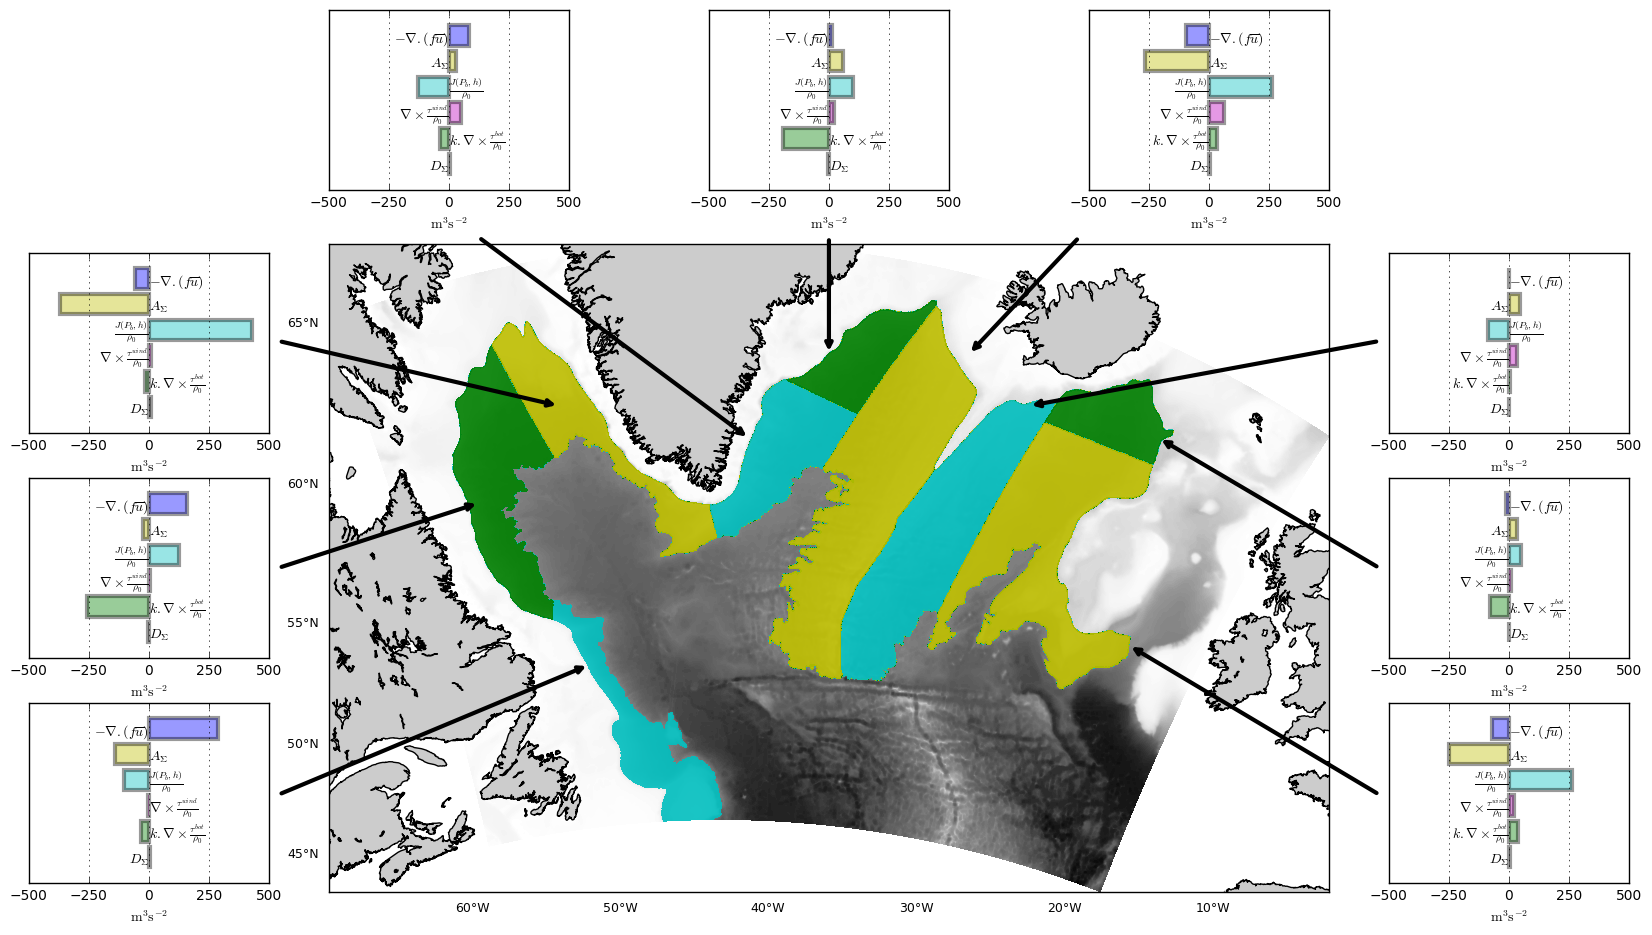
\includegraphics[width=15cm]{./v_b/int_sous_zones_3sv.png}}
\caption{Barotropic vorticity balance integrated on different parts of the gyre near the topography}
\label{bv_zones}
\end{figure}


\end{document}